%%%%%%%%%%%%%%%%%%%%%%%%%%%%%%%%%%%%%%%%%%%%%%%%%%%%%%%%%%%%%%%%%%%%%
%
% VC36O Writeup Template
%
% This is a LaTeX document. LaTeX is a markup language for producing 
% documents. Your task is to fill out this
% document, then to compile this into a PDF document. 
% You will then upload this PDF to `Moodle'.
%
% 
% TO COMPILE:
% > pdflatex thisfile.tex
%
% For references to appear correctly instead of as '??', you must run 
% pdflatex twice.
%
% If you do not have LaTeX and need a LaTeX distribution:
% - Personal laptops (all common OS): www.latex-project.org/get/
%
% If you need help with LaTeX, please come to office hours. 
% Or, there is plenty of help online:
% https://en.wikibooks.org/wiki/LaTeX
%
% Good luck!
%
%%%%%%%%%%%%%%%%%%%%%%%%%%%%%%%%%%%%%%%%%%%%%%%%%%%%%%%%%%%%%%%%%%%%%
%
% How to include two graphics on the same line:
% 
% \includegraphics[\width=0.49\linewidth]{yourgraphic1.png}
% \includegraphics[\width=0.49\linewidth]{yourgraphic2.png}
%
% How to include equations:
%
% \begin{equation}
% y = mx+c
% \end{equation}
% 
%%%%%%%%%%%%%%%%%%%%%%%%%%%%%%%%%%%%%%%%%%%%%%%%%%%%%%%%%%%%%%%%%%%%%%%%%%%%%%%%%%%%%%%%%%%%%%%%

\documentclass[11pt]{article}
\usepackage{float}
\usepackage[english]{babel}
\usepackage[utf8]{inputenc}
\usepackage[colorlinks = true,
            linkcolor = blue,
            urlcolor  = blue]{hyperref}
\usepackage[a4paper,margin=1.5in]{geometry}
\usepackage{stackengine,graphicx}
\usepackage{fancyhdr}
\setlength{\headheight}{15pt}
\usepackage{microtype}
\usepackage{times}
\usepackage{booktabs}
\usepackage{listofitems}
\usepackage{etoolbox}

% Suporte a figuras e subfiguras
\usepackage{graphics}
\usepackage{subfigure}
% From https://ctan.org/pkg/matlab-prettifier
\usepackage[numbered,framed]{matlab-prettifier}

\frenchspacing
\setlength{\parindent}{0cm} % Default is 15pt.
\setlength{\parskip}{0.3cm plus1mm minus1mm}

\pagestyle{fancy}
\fancyhf{}
\lhead{Project Writeup}
\rhead{VC36O 2018/1}
\rfoot{\thepage}

\date{}

\title{\vspace{-1cm}Project 1 Writeup}


\begin{document}
\maketitle
\vspace{-3cm}
\thispagestyle{fancy}

%\section*{Instructions}
%\begin{itemize}
%  \item Describe any interesting decisions you made to write your algorithm.
%  \item Show and discuss the results of your algorithm.
%  \item Feel free to include code snippets, images, and equations.
 % \item Use as many pages as you need, but err on the short side If you feel you only need to write a short amount to meet the brief, th
  
 % \item \textbf{Please make this document anonymous.}
%\end{itemize}

\section*{In the beginning...}
%Ref: http://homepages.dcc.ufmg.br/~william/papers/paper_2003_WICCGPI.pdf
Uma imagem híbrida é a combinação do conteúdo da alta frequência com a baixa frequência de uma mesma imagem. As altas frequências são percebidas à uma distância pequena, pois essas são transmitidas por células retinianas ganglionares P, as quais possuem campos receptivos pequenos, que reagem a pequenos detalhes. Já as baixas frequências são vistas a uma maior distância, pois estimulam as células retinianas ganglionares M que possuem grades campos receptivos, tornando-os quase incapazes de fazer discriminações finas \cite{hibrid}. A Figura~\ref{fig:hibrid} mostra dois exemplos de imagem híbrida, quando vistas de longe a sua expressão é alterada.

\begin{figure}[h]
    \centering
    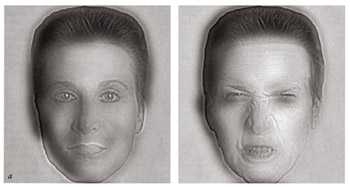
\includegraphics[width=8cm]{hibrid.jpg}
    \caption{Exemplo de imagens híbridas. Fonte: \cite{hibrid}}
    \label{fig:hibrid}
\end{figure}
               
Existem duas formas de criar uma imagem híbrida, no domínio do espaço e uma no domínio da frequência usando a Transformada rápida de Fourier (FFT). A primeira utiliza um filtro gaussiano para obter a baixa frequência, e a subtração da imagem original com a imagem do filtro gaussiano para obter a alta frequência. Já a segunda trabalha com a luminância da imagem, e as imagens de alta e baixa frequências são obtidas sem esforço computacional necessário utilizando um método FFT, baseado na decomposição  do  núcleo  da  transformada  em  matrizes  esparsas \cite{William}.

Para a criação da imagem híbrida, foi utilizado a linguagem Octave, nos quais as duas formas de criar essas imagens foram implementadas (com e sem a FFT). Parte do código já foi disponibilizado pronto, tal como, o filtro gaussiano e a o cálculo da FFT. Dessa forma, o primeiro passo foi de entender o funcionamento dos mesmos.

Depois de compreender o código e acrescentar o que faltava para sua conclusão, foram geradas duas imagens híbridas, a primeira de um gato (Figura~\ref{fig:cat}) e cachorro (Figura~\ref{fig:dog}) fornecida junto com o código fonte, e a segunda de duas teclas numéricas do notebook (8 e 9), nas quais foram tiradas e editadas no editor de imagens Gimp\footnote{https://www.gimp.org/}. A imagem original do teclado é demostrada na Figura~\ref{fig:teclado}, já as editadas na Figura~\ref{fig:teclas}.

\begin{figure}[h]
    \centering
    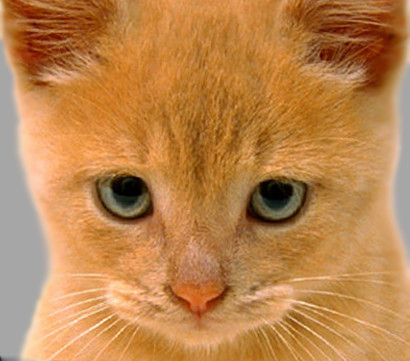
\includegraphics[width=4cm]{cat.jpg}
    \caption{Imagem utilizada para alta frequência}
    \label{fig:cat}
\end{figure}

\begin{figure}[h]
    \centering
    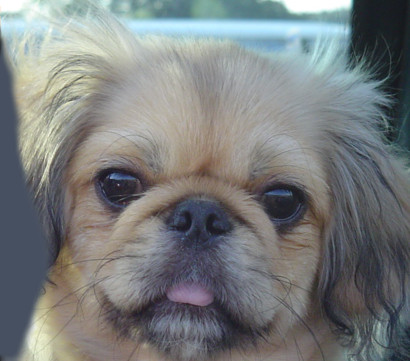
\includegraphics[width=4cm]{dog.jpg}
    \caption{Imagem utilizada para baixa frequência}
    \label{fig:dog}
\end{figure}

\begin{figure}[H]
    \centering
    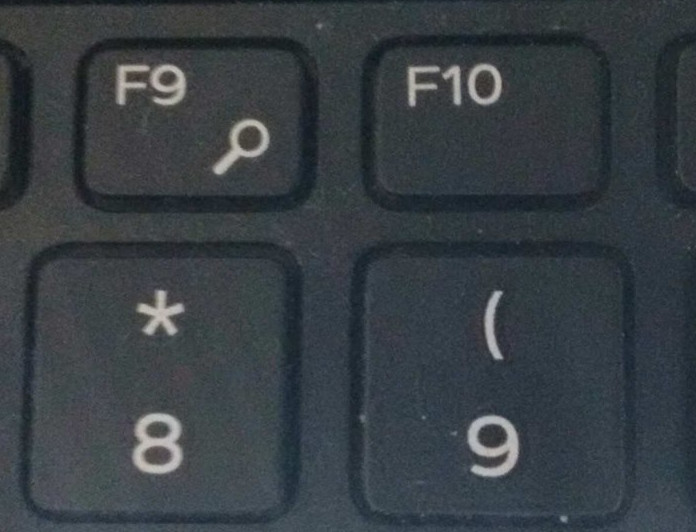
\includegraphics[width=4cm]{num.jpg}
    \caption{Imagem tirada do teclado numérico do notebook}
    \label{fig:teclado}
\end{figure}

\begin{figure}[ht]
	\centering
	\subfigure[Imagem editada do teclado]{
	    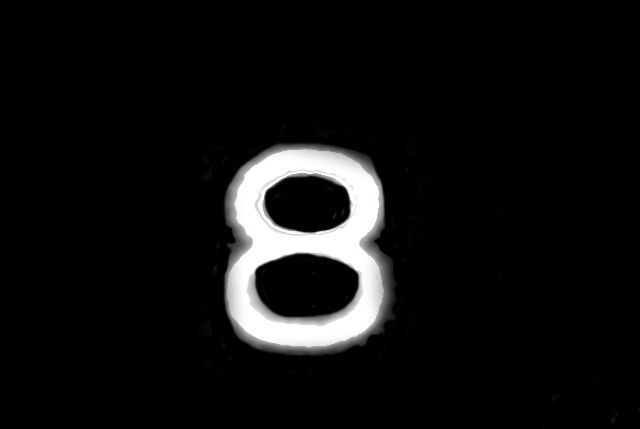
\includegraphics[height=2.5cm]{num1.jpg}
	    \label{fig:subfig1}
	}
	\subfigure[Imagem editada do teclado]{
		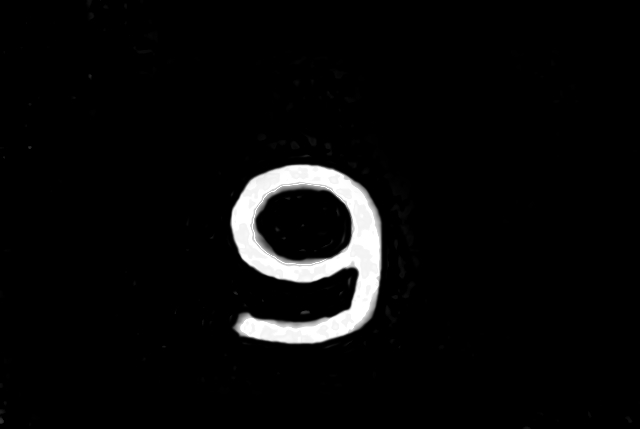
\includegraphics[height=2.5cm]{num2.jpg}
	    \label{fig:subfig2}
	}
	\caption[]{ \subref{fig:subfig1} Alta frequência e \subref{fig:subfig2} Baixa frequência }
	\label{fig:teclas}
\end{figure}

As imagens da tecla 8 e 9 foram saturadas e preenchidas com cores preto e braco, de forma que os números pudessem ficar sobrepostos para obter o melhor resultado possível. As próximas seções irão mostrar parte das implementações e os resultados obtidos.

\section*{Interesting Implementation Detail}


Na implementação da geração de imagem híbrida sem utilização da transformada rápida de Fourier, é descrito a parte modificada do arquivo \texttt{gen\textunderscore hybrid\textunderscore image.m}, que está descrito abaixo:

\begin{lstlisting}[style=Matlab-editor]
function [hybrid_image, low_frequencies, high_frequencies] = gen_hybrid_image(image1, image2, cutoff_frequency)

filter = fspecial('Gaussian', cutoff_frequency*4+1, cutoff_frequency);
low_frequencies = my_imfilter(image1, filter);

high_frequencies = image2 - my_imfilter(image2, filter);

hybrid_image = low_frequencies + high_frequencies;
\end{lstlisting}

Na linha três é criado um filtro Gaussiano, na linha quatro é aplicado esse filtro, e consequentemente é obtido a imagem somente com as baixas frequências. Já na linha seis são adquiridas as altas frequências por meio da subtração da imagem dois original pela imagem dois após a aplicação do filtro que foi criado na linha quatro. Por fim, na linha oito é feito a criação da imagem híbrida com a junção da imagem de baixa frequência com a imagem de alta frequência. 



Já na geração da imagem híbrida usando a FFT, são evidenciados 
alguns detalhes de como as baixas e altas frequências da imagem foram obtidas, no qual está implementado no arquivo \texttt{gen\textunderscore hybrid\textunderscore image\textunderscore fft.m}. A seguir está descrito parte do código para obter apenas a baixa frequência.

\begin{lstlisting}[style=Matlab-editor]
% Cria um padding
b = padarray(image1, size(image1), "zeros", "post");

% Converte para double
c = im2double(b(:, :, 1:3));

%Faz o padding da imagem
d = fft2(c);

%Centraliza a transformada de fourier
d = fftshift(d);

% Pega as dimensoes da vaariavel c
[n m o] = size(c);

% Faz uma matriz de zeros com as dimensoes de n e m
h = zeros([n, m]);

%Construindo o filtro passa-baixa
for i = 1:n
  for j = 1:m
    h(i, j) = H(i, j, size(c), cutoff_frequency);
  end
end

% Multiplicando a matriz de transformada de Fourier pelo filtro
g = d.*h;

% Descentralizando a matriz
g = ifftshift(g);

% Aplicando a transformada inversa rapida
at = ifft2(g);

% Tira os valores negativos de at
at = abs(at);

% Pega as dimensoes da imagem 1
[x y o] = size(image1);

% Extrai da regiao X e Y
atc = at(1:x, 1:y, :);

% Atribuindo a imagem final
low_frequencies = atc;

\end{lstlisting}

A transformada de Fourier é criada nas linhas 8, 9, 10 e nos laços da linha 14, 15 e 16 é criado o filtro para a baixa frequência. O objetivo é centralizar a transformada de forma que seu centro fique branco e o resto preto. A transformada e o filtro são multiplicados na lina 20. Os valores negativos da transformada são tirados na linha 27, e extraída a região X e Y da imagem na linha 32. Por fim, a baixa frequência, na linha 34, será a região X e Y, que irá gerar uma imagem borrada.

Para a alta frequência a mesma ideia é seguida, gerar a transformada e criar o filtro baixa frequência. Porém, esse filtro deve ser invertido para que seu resultado seja de alta frequência. A seguir está descrito parte do código pra a obtenção da alta frequência da imagem.

\begin{lstlisting}[style=Matlab-editor]
% Cria um padding
b = padarray(image2, size(image2), "zeros", "post");

% Converte para double
c = im2double(b(:, :, 1:3));

%Faz o padding da imagem
d = fft2(c);

%Centraliza a transformada de fourier
d = fftshift(d);

% Pega as dimensoes da vaariavel c
[n m o] = size(c);

% Faz uma matriz de zeros com as dimensoes de n e m
h = zeros([n, m]);

%Construindo o filtro passa-alta
for i = 1:n
  for j = 1:m
    h(i, j) = H(i, j, size(c), cutoff_frequency);
  end
end

% Inverter a transformada
invert = ones(size(im2uint8(h)));
h = invert .- h;

% Multiplicando a matriz de transformada de Fourier pelo filtro
g = d.*h;

% Descentralizando a matriz
g = ifftshift(g);

% Aplicando a transformada inversa rapida
at = ifft2(g);

% Pega as dimensoes da imagem 2
[x y o] = size(image2);

% Extrai da regiao X e Y
atc = at(1:x,1:y, :);

% Atribuindo a imagem final
high_frequencies = atc;
\end{lstlisting}


As linhas 20 e 21 são as que diferem do código da alta para baixa frequência. Ao criar uma matriz contendo apenas valores 1 e a subtrair pelo filtro obtido, irá criar o filtro de alta frequência, na qual o seu centro irá possui valores em zero e o resto valores em um. Por fim, para obter a imagem híbrida, basta fazer o módulo da soma da imagem de baixa com alta frequência, como descrito a seguir:


\begin{lstlisting}[style=Matlab-editor]
%%%%%%%%%%%%%%%%%%%%%%%%%%%%%%%%%%%%%%%%%%%%%%%%%%
% Combine the high frequencies and low frequencies
%%%%%%%%%%%%%%%%%%%%%%%%%%%%%%%%%%%%%%%%%%%%%%%%%%
hybrid_image = abs(low_frequencies + high_frequencies);
\end{lstlisting}

\section*{A Result}

Os resultados obtidos na criação da imagem híbrida do gato e cachorro, tanto no domínio do espaço (sem FFT) como no da frequência, foram os esperados. As altas frequências obtidas são demonstradas na Figura~\ref{fig:altas}, já as baixas frequências na Figura~\ref{fig:baixas}, por fim a imagem híbrida está demonstrada nas Fgura~\ref{fig:final}, \ref{fig:gen_hybrid_image_scales} e \ref{fig:gen_hybrid_image_scales_fft}.

\begin{figure}[ht]
	\centering
	\subfigure[]{
	    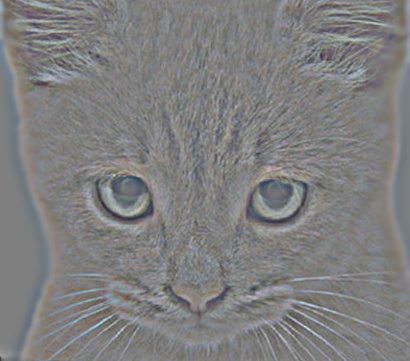
\includegraphics[height=2.5cm]{gen_hybrid_image/high_frequencies.jpg}
	    \label{fig:alta1}
	}
	\subfigure[]{
		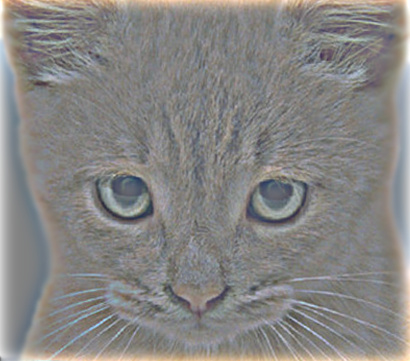
\includegraphics[height=2.5cm]{gen_hybrid_image/high_frequencies_fft.jpg}
	    \label{fig:alta2}
	}
	\caption[]{ \subref{fig:alta1} Alta frequência gerada pelo domínio do espaço \subref{fig:alta2} Alta frequência gerada pela FFT}
	\label{fig:altas}
\end{figure}
 
 \begin{figure}[ht]
 	\centering
 	\subfigure[]{
 	    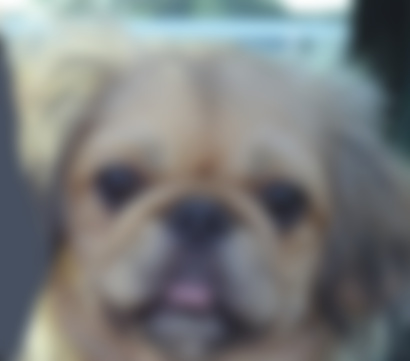
\includegraphics[height=2.5cm]{gen_hybrid_image/low_frequencies.jpg}
 	    \label{fig:baixa1}
 	}
 	\subfigure[]{
 		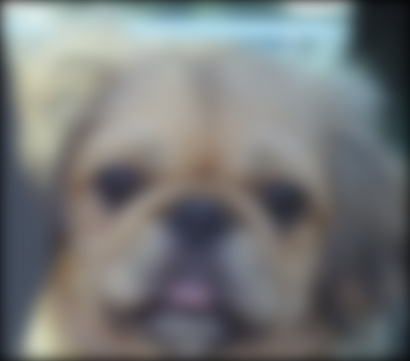
\includegraphics[height=2.5cm]{gen_hybrid_image/low_frequencies_fft.jpg}
 	    \label{fig:baixa2}
 	}
 	\caption[]{ \subref{fig:alta1} Baixa frequência gerada pelo domínio do espaço \subref{fig:alta2} Baixa frequência gerada pela FFT}
 	\label{fig:baixas}
 \end{figure}
 
 
 \begin{figure}[H]
    \centering
    \subfigure[]{
    	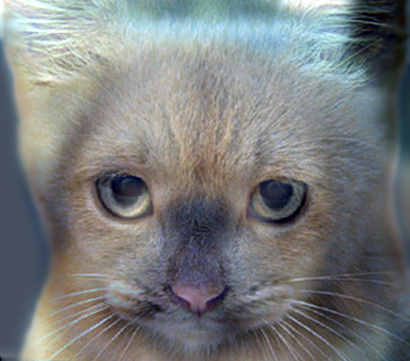
\includegraphics[width=2.5cm]{gen_hybrid_image/hybrid_image.jpg}
    	\label{fig:gen_hybrid_image1}
    }
    \subfigure[]{
        	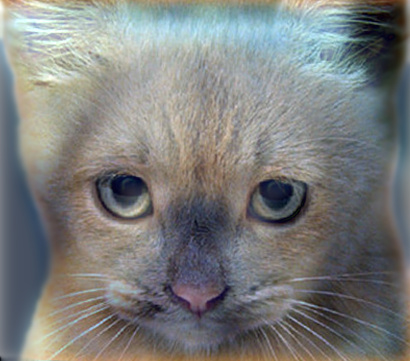
\includegraphics[width=2.5cm]{gen_hybrid_image/hybrid_image_fft.jpg}
        	\label{fig:gen_hybrid_image2}
        }
    \caption[]{\subref{fig:gen_hybrid_image1} Imagem híbrida final obtida sem FFT {\subref{fig:gen_hybrid_image2} Imagem híbrida final obtida com FFT}}
    \label{fig:final}
\end{figure}

\begin{figure}[H]
    \centering
    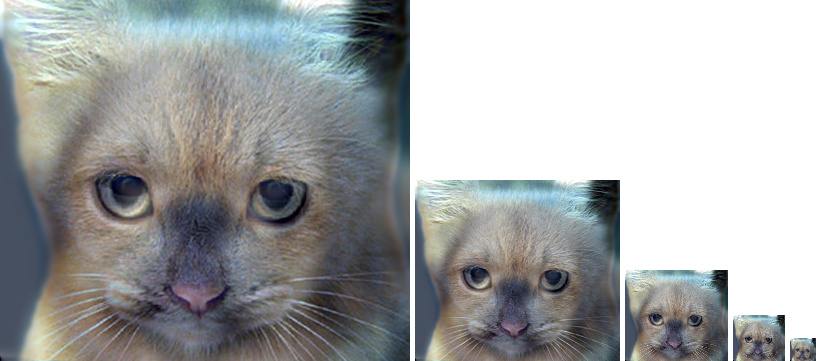
\includegraphics[width=5cm]{gen_hybrid_image/hybrid_image_scales.jpg}
    \caption{Escalas das imagens híbridas obtidas sem FFT}
    \label{fig:gen_hybrid_image_scales}
\end{figure}

\begin{figure}[H]
    \centering
    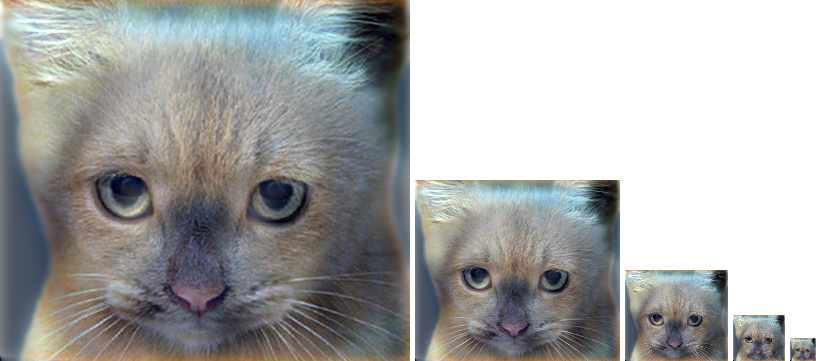
\includegraphics[width=5cm]{gen_hybrid_image/hybrid_image_scales_fft.jpg}
    \caption{Escalas das imagens híbridas obtidas pela FFT}
    \label{fig:gen_hybrid_image_scales_fft}
\end{figure}

Já os resultados obtidos na criação da imagem híbrida dos números oito e nove, tanto no domínio do espaço (sem FFT) como no da frequência, foram razoavelmente bons. As altas frequências obtidas são demonstradas na Figura~\ref{fig:altasNum}, já as baixas frequências na Figura~\ref{fig:baixasNum}, por fim a imagem híbrida está demonstrada nas Fgura~\ref{fig:finalNum}, \ref{fig:gen_hybrid_image_scalesNum} e \ref{fig:gen_hybrid_image_scalesNum2}.

Para obter a imagem final dos números utilizando a transformada de Fourier, foi necessário realizar uma alteração no código, pois tais imagens estão na escala cinza e apresentam uma dimensão menor. Para isso, tirou-se \texttt{(:, :, 1:3)} das linhas 4 do código \texttt{gen\_hybrid\_image\_fft} da baixa e alta frequência descrito na linha anterior.

\begin{figure}[ht]
	\centering
	\subfigure[]{
	    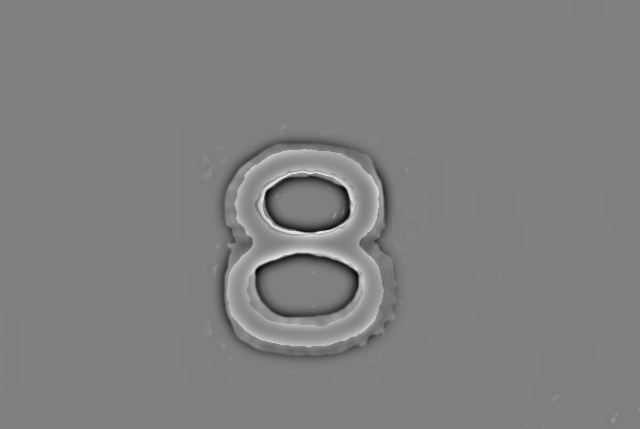
\includegraphics[height=2.5cm]{numeros/high_frequencies.jpg}
	    \label{fig:altaNum1}
	}
	\subfigure[]{
		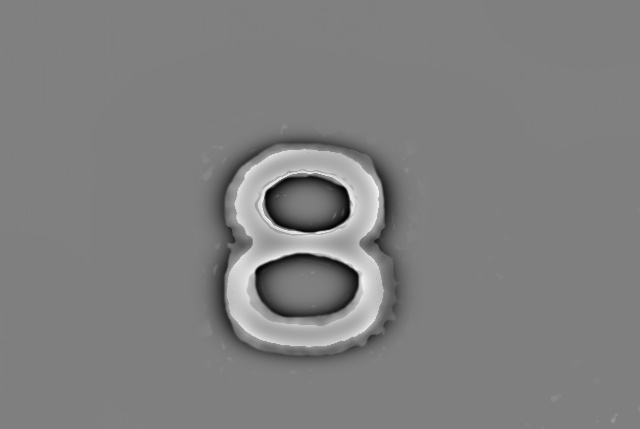
\includegraphics[height=2.5cm]{numeros/high_frequencies_fft.jpg}
	    \label{fig:altaNum2}
	}
	\caption[]{ \subref{fig:altaNum1} Alta frequência gerada pelo domínio do espaço \subref{fig:altaNum2} Alta frequência gerada pela FFT}
	\label{fig:altasNum}
\end{figure}


 \begin{figure}[ht]
 	\centering
 	\subfigure[]{
 	    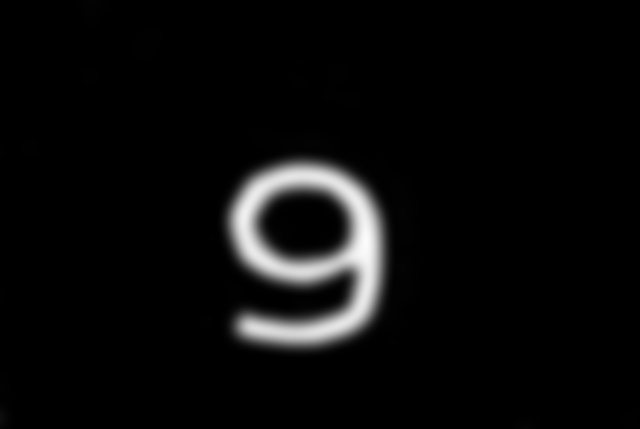
\includegraphics[height=2.5cm]{numeros/low_frequencies.jpg}
 	    \label{fig:baixaNum1}
 	}
 	\subfigure[]{
 		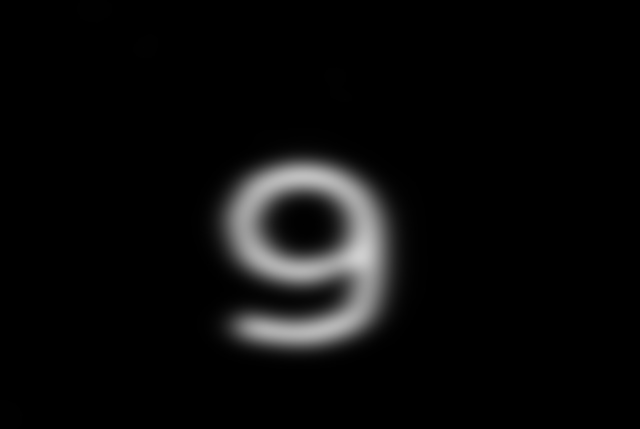
\includegraphics[height=2.5cm]{numeros/low_frequencies_fft.jpg}
 	    \label{fig:baixaNum2}
 	}
 	\caption[]{ \subref{fig:altaNum1} Baixa frequência gerada pelo domínio do espaço \subref{fig:altaNum2} Baixa frequência gerada pela FFT}
 	\label{fig:baixasNum}
 \end{figure}


\begin{figure}[H]
    \centering
    \subfigure[]{
    	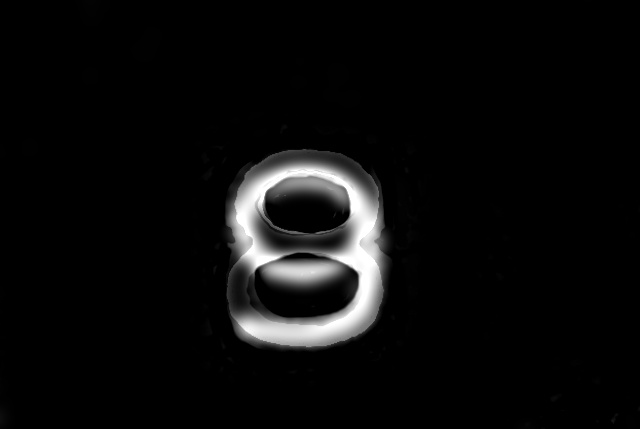
\includegraphics[width=3.5cm]{numeros/hybrid_image.jpg}
    	\label{fig:gen_hybrid_imageNum1}
    }
    \subfigure[]{
        	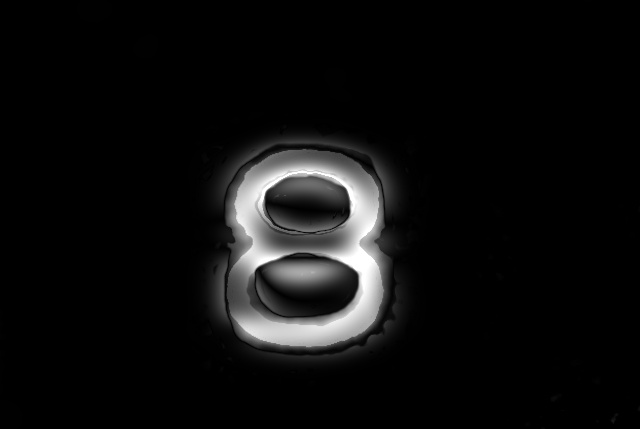
\includegraphics[width=3.5cm]{numeros/hybrid_image_fft.jpg}
        	\label{fig:gen_hybrid_imageNum2}
        }
    \caption[]{\subref{fig:gen_hybrid_imageNum1} Imagem híbrida final obtida sem FFT {\subref{fig:gen_hybrid_imageNum2} Imagem híbrida final obtida com FFT}}
    \label{fig:finalNum}
\end{figure}



\begin{figure}[H]
    \centering
    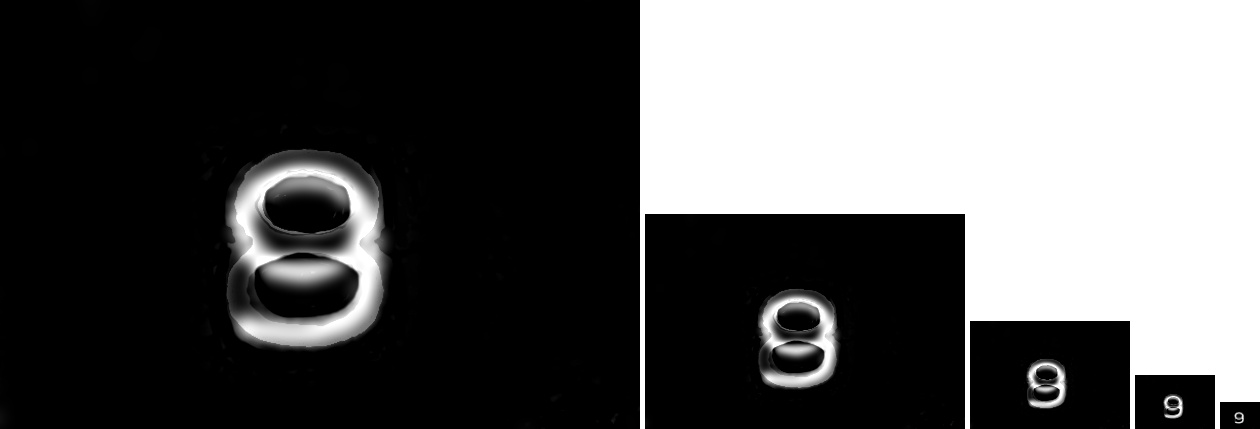
\includegraphics[width=7cm]{numeros/hybrid_image_scales.jpg}
    \caption{Escalas das imagens híbridas obtidas sem FFT}
    \label{fig:gen_hybrid_image_scalesNum}
\end{figure}

\begin{figure}[H]
    \centering
    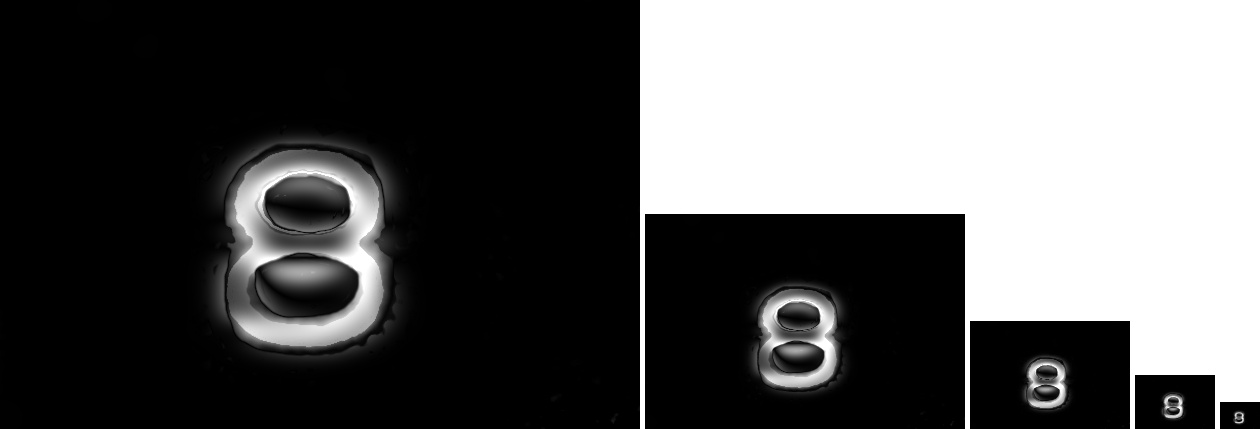
\includegraphics[width=7cm]{numeros/hybrid_image_scales_fft.jpg}
    \caption{Escalas das imagens híbridas obtidas com FFT}
    \label{fig:gen_hybrid_image_scalesNum2}
\end{figure}

\bibliographystyle{abntex2-alf}

\bibliography{references}

\end{document}
